% !TeX root = ../../Book1.tex
\section{混合性与典型模型}
\label{b1:sec:3205}

遍历性决定长期平均是否化成一个空间积分。
还可以提出更强的问题：在时刻零观察到一个事件之后，经过很长时间，
这个信息对另一个事件的发生概率是否仍有影响？
混合性考察的正是这种相隔很久的相关，而不先把各个时刻取平均。
本节从集合的相交概率出发，再用圆周上的两个具体映射比较两种性质。

\subsection{混合性的定义}
\label{b1:subsec:320501}

设初始状态 \(x\) 按概率测度 \(\mu\) 分布。
事件“现在位于 \(A\)”写成 \(x\in A\)，
事件“\(n\) 步之后位于 \(B\)”写成 \(x\in T^{-n}B\)。
因此两件事同时发生的概率是 \(\mu(A\cap T^{-n}B)\)。
这里使用的是逆像，即使 \(T\) 没有逆映射，这个集合仍有明确意义。

\begin{definition}[混合性]
\label{b1:def:mixing-32}
设 \((X,\mathcal A,\mu)\) 为概率空间，\(T:X\to X\) 为可测保测变换。
若对每两个固定的 \(A,B\in\mathcal A\)，都有
\begin{equation}
 \lim_{n\to\infty}\mu(A\cap T^{-n}B)=\mu(A)\cdot\mu(B),
 \label{b1:eq:mixing-sets-32}
\end{equation}
则称 \(T\) 关于 \(\mu\) 具有\term[hunhexing]{混合性}[mixing]，
也称 \(T\) 是混合的。本节的“混合”指强混合。
\end{definition}
\termidx[qiang-hunhe]{强混合}
\foreignidx{strong mixing}

强混合这一名称见叶向东、黄文、邵松《遍历理论及其应用》2023年稿的
\(\S2.4\)，用于区别另一种先对相关误差的绝对值取时间平均的弱混合条件。
\eqref{b1:eq:mixing-sets-32}要求相关误差本身趋零；弱混合则要求这些误差的绝对值在时间平均下趋零。

\ProseParagraphBreak

若 \(\mu(A)>0\)，定义可改写为
\[
 \frac{\mu(A\cap T^{-n}B)}{\mu(A)}\longrightarrow\mu(B).
\]
左端是在已知起点属于 \(A\) 时，\(n\) 步后进入 \(B\) 的条件概率。
混合性说这种条件影响在极限中消失，而不是说有限时刻就已经独立。
“每两个固定的集合”也不意味着对所有集合一致收敛；
随 \(n\) 改变事件，可能保留完全不同的相关。

\begin{proposition}[混合性的函数判别]
\label{b1:prop:mixing-correlations-32}
设 \((X,\mathcal A,\mu)\) 为概率空间，\(T:X\to X\) 为可测保测变换。
则 \(T\) 混合，当且仅当对任意 \(f,g\in L^2(\mu;\mathbb C)\)，都有
\begin{equation}
 \int_X(f\circ T^n)\cdot\overline g\,\mathrm d\mu
 \longrightarrow
 \left(\int_Xf\,\mathrm d\mu\right)
 \overline{\left(\int_Xg\,\mathrm d\mu\right)}.
 \label{b1:eq:mixing-correlation-32}
\end{equation}
也可以只要求对所有实值 \(L^2\) 函数成立，此时省略复共轭。
\end{proposition}
\begin{proof}
取 \(f=\mathbf1_B\)、\(g=\mathbf1_A\)，函数条件就给出集合条件。
反过来，假设 \(T\) 混合。先把 \(f,g\) 都取为有限值简单函数，
逐项展开积分并使用\eqref{b1:eq:mixing-sets-32}，就得到所需极限。
复系数的展开中，\(g\) 的系数取共轭。

对一般 \(f,g\in L^2\)，用简单函数 \(u,v\) 分别逼近。
Cauchy--Schwarz 不等式及保测性给出对所有 \(n\) 同时成立的界
\[
 \begin{aligned}
 &\left|\int_X(f\circ T^n)\cdot\overline g\,\mathrm d\mu
       -\int_X(u\circ T^n)\cdot\overline v\,\mathrm d\mu\right|\\
 &\hspace{1em}\leq
 \|f-u\|_2\cdot\|g\|_2+\|u\|_2\cdot\|g-v\|_2.
 \end{aligned}
\]
由于 \(\mu(X)=1\)，还有 \(\|w\|_1\leq\|w\|_2\)；
故两个积分乘积的差也不超过右端同一个量。
先令 \(n\to\infty\)，简单函数的相关误差趋零。
再选 \(u,v\) 使两项逼近误差任意小，就得到一般函数的结论。
若开始只假设实值函数条件，实、虚部展开同样给出复值版本。
\end{proof}

式\eqref{b1:eq:mixing-correlation-32}只说相关积分收敛，不说 \(f\circ T^n\) 在范数中趋于常函数。
例如，若 \(\int_Xf\,\mathrm d\mu=0\)，保测性仍给出
\(\|f\circ T^n\|_2=\|f\|_2\)。当 \(f\ne0\) 时，这个范数不会趋零。
混合性使它对每个固定测试函数的相关趋零，与保留自身范数并不矛盾。

\subsection{混合蕴含遍历}
\label{b1:subsec:320502}

若一个正测度集合永远保持不变，则知道起点在其中，
就永远知道后续状态也在其中。这种永久信息会妨碍混合。
下面的证明把这一想法写成一个等式，并且兼容模零不变的约定。

\begin{proposition}[混合蕴含遍历]
\label{b1:prop:mixing-ergodic-32}
设 \((X,\mathcal A,\mu)\) 为概率空间，\(T:X\to X\) 为可测保测变换。
若 \(T\) 关于 \(\mu\) 混合，则 \(T\) 关于 \(\mu\) 遍历。
\end{proposition}
\begin{proof}
取 \(E\in\mathcal A\)，满足 \(\mu(T^{-1}E\triangle E)=0\)。
由
\[
 T^{-n}E\triangle E
 \subseteq\bigcup_{j=0}^{n-1}T^{-j}(T^{-1}E\triangle E)
\]
及保测性，得到 \(\mu(T^{-n}E\triangle E)=0\)。
于是对每个 \(n\)，\(\mu(E\cap T^{-n}E)=\mu(E)\)。
混合性又要求左端趋于 \(\mu(E)^2\)，所以
\(\mu(E)=\mu(E)^2\)，即 \(\mu(E)\in\{0,1\}\)。
\end{proof}

反向蕴含不成立。先看有限等概率空间中的一个长度为 \(q\geq2\) 的循环。
它是遍历的，但对单点集 \(E\)，
\[
 \mu(E\cap T^{-n}E)=
 \begin{cases}
  1/q,&q\mid n,\\
  0,&q\nmid n.
 \end{cases}
\]
这个序列并不趋于 \(1/q^2\)。平均访问频率可以稳定，
单个时刻的相关却仍保留周期振荡。
无理圆周转动没有有限周期，但也不混合；下一小节将解释阻碍在哪里。

\subsection{圆周转动的遍历与非混合}
\label{b1:subsec:320503}

把圆周写作 \(\mathbb T=\mathbb R/\mathbb Z\)，以 \([0,1)\) 为代表，
配备 Borel \(\sigma\)-代数及归一化长度测度 \(m\)。
对 \(\alpha\in\mathbb R\)，令
\[
 R_\alpha x=x+\alpha\bmod1.
\]
\secref{b1:sec:3201}已经用分段换元证明 \(R_\alpha\) 保测。
无理转动的稠密性与集合的平移连续性将相互配合，把对一个转角的不变性传给所有转角。

\begin{lemma}[无理转动的稠密性与集合的平移连续性]
\label{b1:lem:rotation-density-continuity-32}
在圆周 \(\mathbb T\) 及其归一化长度测度 \(m\) 上，有以下两条结论。
\begin{enumerate}
\item\label{b1:item:rotation-dense-group-32}
若 \(\alpha\notin\mathbb Q\)，则
\(\{k\alpha\bmod1:k\in\mathbb Z\}\) 在圆周中稠密。
\item\label{b1:item:rotation-translation-32}
对每个 Borel 集 \(E\subseteq\mathbb T\)，有
\[
 \|\mathbf1_E\circ R_t-\mathbf1_E\|_{L^1(m)}
 =m(R_t^{-1}E\triangle E)\longrightarrow0
 \quad\text{当 }t\to0\bmod1.
\]
\end{enumerate}
\end{lemma}
\begin{proof}
给定正整数 \(M\)，把 \([0,1)\) 分成 \(M\) 个等长半开区间。
\(M+1\) 个不同的点 \(0,\alpha,\ldots,M\alpha\bmod1\)
中至少两个落在同一区间。把两个代表相减，必要时交换次序，得到
\[
 0<\beta<1/M,\quad \beta=\ell\alpha\bmod1
\]
及某个非零整数 \(\ell\)。对每个 \(t\in[0,1)\)，取
\(j=\lfloor t/\beta\rfloor\)，便有 \(0\leq t-j\beta<\beta\)，
且 \(j\beta<1\) 是该循环子群中的元素。
令 \(M\) 任意大，证明了稠密性。这里得到的是正负整数迭代组成的循环子群的稠密性；下面用平移连续性把这种逼近用于可测集。

对第二条，先设 \(E\) 是 \(r\) 个区间的并。
每个区间平移小量 \(t\) 后，只在其两个端点附近发生差异，
所以对足够小的实数代表 \(t\)，
\[
 m(R_t^{-1}E\triangle E)\leq2r|t|.
\]
一般 Borel 集可以在对称差测度下用有限个区间的并 \(J\) 逼近。
具体地，先由 Lebesgue 外正则性取开集 \(O\supseteq E\)，
使 \(m(O\setminus E)<\varepsilon\)；
把 \(O\) 写成至多可数个区间的并，截取有限多个，使剩余长度小于 \(\varepsilon\)，
便有 \(m(E\triangle J)<2\varepsilon\)。
平移保测与三角不等式于是给出
\[
 \begin{aligned}
 m(R_t^{-1}E\triangle E)
 &\leq m(R_t^{-1}E\triangle R_t^{-1}J)
       +m(R_t^{-1}J\triangle J)+m(J\triangle E)\\
 &\leq4\varepsilon+2r|t|.
 \end{aligned}
\]
先令 \(t\to0\)，再令 \(\varepsilon\to0\)，即得结论。
\end{proof}

上面第二条补足了一个不能省略的桥梁：
一个集合即使在稠密子群的作用下不变，也不能仅凭“稠密”就对每个点取极限。
示性函数未必连续；允许把群元素的逼近传给函数的，是 \(L^1\) 平移连续性。

\begin{theorem}[圆周转动的遍历性]
\label{b1:thm:irrational-rotation-32}
在 \((\mathbb T,\mathcal B(\mathbb T),m)\) 上，
转动 \(R_\alpha x=x+\alpha\bmod1\) 遍历，当且仅当 \(\alpha\notin\mathbb Q\)。
无论 \(\alpha\) 是否有理，\(R_\alpha\) 都不是混合的。
\end{theorem}
\begin{proof}
先设 \(\alpha\) 无理。取模零不变的 Borel 集 \(E\)，即
\(\mathbf1_E\circ R_\alpha=\mathbf1_E\) 于 \(L^1(m)\)。
转动可逆且两个方向都保测，故这个等式对每个整数倍 \(k\alpha\) 仍成立。
给定任意 \(t\in\mathbb T\)，取 \(k_j\alpha\to t\bmod1\)。
由上一引理的平移连续性与平移等距性，
\[
 \|\mathbf1_E\circ R_t-\mathbf1_E\|_1
 \leq\|\mathbf1_E\circ R_t-\mathbf1_E\circ R_{k_j\alpha}\|_1
 \longrightarrow0.
\]
所以对每个 \(t\)，该范数都是零。

不能据此直接说对所有 \(t,x\) 等式同时成立。
应对非负 Borel 函数 \((x,t)\mapsto|\mathbf1_E(x+t)-\mathbf1_E(x)|\)
使用 Tonelli 定理：
\[
 \int_{\mathbb T}\int_{\mathbb T}
 |\mathbf1_E(x+t)-\mathbf1_E(x)|\,\mathrm dm(x)\,\mathrm dm(t)=0.
\]
交换次序后，对几乎每个 \(x\)，内层关于 \(t\) 的积分为零，
从而 \(\mathbf1_E(x+t)=\mathbf1_E(x)\) 对几乎每个 \(t\) 成立。
再对 \(t\) 积分，得到
\[
 \mathbf1_E(x)=\int_{\mathbb T}\mathbf1_E(x+t)\,\mathrm dm(t)=m(E)
 \quad\text{对几乎每个 }x.
\]
这迫使 \(m(E)\) 为零或一，证明遍历性。

若 \(\alpha=p/q\)，其中 \(p\in\mathbb Z\)、\(q\geq1\)，取
\[
 E=\{\,x\in[0,1):qx\bmod1\in[0,1/2)\,\}.
\]
它由 \(q\) 个长度为 \(1/(2q)\) 的区间组成，故 \(m(E)=1/2\)；
而 \(qR_\alpha x=qx+p\bmod1\)，所以 \(E\) 严格不变。
因此有理转动不遍历。

最后，对任意 \(\alpha\)，取 \(u(x)=\exp(2\pi\mathrm ix)\)。
直接积分得 \(\int_{\mathbb T}u\,\mathrm dm=0\)，且
\[
 u(R_\alpha^nx)=e^{2\pi\mathrm in\alpha}\cdot u(x),\quad
 \int_{\mathbb T}(u\circ R_\alpha^n)\cdot\overline u\,\mathrm dm
 =e^{2\pi\mathrm in\alpha}.
\]
右端的模恒为一，不可能趋零，与混合性的函数判别矛盾。
\end{proof}

无理转动的相关中保留了一个始终存在的相位。
对同一个函数 \(u(x)=e^{2\pi\mathrm ix}\)，其时间平均却满足
\[
 A_Nu(x)=e^{2\pi\mathrm ix}
 \frac{1-e^{2\pi\mathrm iN\alpha}}{N(1-e^{2\pi\mathrm i\alpha})},
 \quad
 \|A_Nu\|_\infty\leq\frac2{N|1-e^{2\pi\mathrm i\alpha}|}
 \longrightarrow0.
\]
相位自身没有衰减，但取时间平均后可以抵消。
这个计算说明遍历平均的收敛与单次相关的衰减是不同的问题；
其中的速度依赖这个具体观测函数，不能推给任意 \(L^1\) 函数。

\subsection{倍增映射的混合性}
\label{b1:subsec:320504}

仍在 \([0,1)\) 上使用 Borel \(\sigma\)-代数与长度概率测度 \(m\)，令
\[
 D(x)=2x\bmod1.
\]
它把左右两半各自拉伸为整个区间。虽然每个分支把长度扩大两倍，
每个目标集合恰有两个分支的逆像，逆像的总长度仍保持不变。
\cref{b1:fig:doubling-map-32}把两个分支及同一目标区间的逆像画在一起。

\begin{figure}[htbp]
\centering
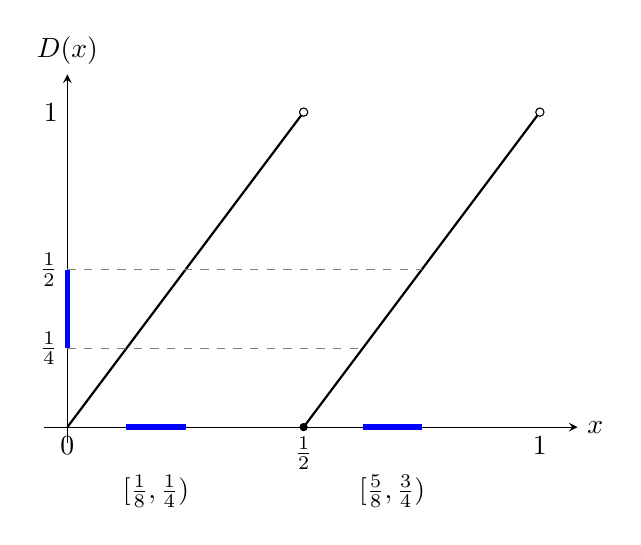
\begin{tikzpicture}[x=6cm,y=4cm,>=stealth]
 \draw[->] (-.05,0)--(1.08,0) node[right]{\(x\)};
 \draw[->] (0,-.05)--(0,1.12) node[above]{\(D(x)\)};
 \draw[thick] (0,0)--(.5,1);
 \draw[thick] (.5,0)--(1,1);
 \draw[fill=white] (.5,1) circle[radius=1.5pt];
 \draw[fill=white] (1,1) circle[radius=1.5pt];
 \fill (.5,0) circle[radius=1.5pt];
 \draw[dashed,gray] (0,.25)--(.625,.25);
 \draw[dashed,gray] (0,.5)--(.75,.5);
 \draw[line width=2pt,blue] (0,.25)--(0,.5);
 \draw[line width=2pt,blue] (.125,0)--(.25,0);
 \draw[line width=2pt,blue] (.625,0)--(.75,0);
 \node[left] at (0,.25){\(\frac14\)};
 \node[left] at (0,.5){\(\frac12\)};
 \node[left] at (0,1){\(1\)};
 \node[below] at (0,0){\(0\)};
 \node[below] at (.5,0){\(\frac12\)};
 \node[below] at (1,0){\(1\)};
 \node[below] at (.1875,-.12){\([\frac18,\frac14)\)};
 \node[below] at (.6875,-.12){\([\frac58,\frac34)\)};
\end{tikzpicture}
\caption[倍增映射及区间的两个逆像]{倍增映射及区间的两个逆像。
蓝色目标区间为 \([1/4,1/2)\)，其两个逆像各长 \(1/8\)，总长仍为 \(1/4\)。
分支顶端的空心点表示该端点不属于相应分支。}
\label{b1:fig:doubling-map-32}
\end{figure}

迭代 \(n\) 次后，\(D^n(x)=2^nx\bmod1\) 有 \(2^n\) 个这样的分支。
每个长度 \(2^{-n}\) 的二进区间都被拉伸为整个 \([0,1)\)。
因此，一个只分辨到较粗二进尺度的初始事件，
在足够晚的时刻会与任意固定目标事件精确独立，而不仅仅是近似独立。

\begin{lemma}[二进区间上的精确相关]
\label{b1:lem:dyadic-independence-32}
设 \(D(x)=2x\bmod1\) 作用于 \([0,1)\) 上的 Borel 概率空间与长度测度 \(m\)。
对整数 \(r\geq0\)、\(0\leq j<2^r\)，令
\[
 I_{r,j}=[j2^{-r},(j+1)2^{-r}).
\]
则对任意 Borel 集 \(B\subseteq[0,1)\) 以及整数 \(n\geq r\)，
\[
 m(I_{r,j}\cap D^{-n}B)=2^{-r}m(B).
\]
若 \(A\) 是若干个同级 \(I_{r,j}\) 的并，则
\(m(A\cap D^{-n}B)=m(A)\cdot m(B)\) 对 \(n\geq r\) 成立。
\end{lemma}
\begin{proof}
把 \(I_{r,j}\) 划分成 \(2^{n-r}\) 个 \(n\) 级区间
\(J_\ell=[\ell2^{-n},(\ell+1)2^{-n})\)。
在每个 \(J_\ell\) 上，\(D^n(x)=2^nx-\ell\)，
故 \(J_\ell\cap D^{-n}B=(B+\ell)/2^n\)，其测度为 \(2^{-n}m(B)\)。
把这些互不相交的部分相加，得到
\(2^{n-r}\cdot2^{-n}m(B)=2^{-r}m(B)\)。
若 \(A\) 含有多个 \(r\) 级区间，再利用有限可加性即可。
\end{proof}

\begin{theorem}[倍增映射的混合性]
\label{b1:thm:doubling-mixing-32}
区间 \([0,1)\) 上的倍增映射 \(D(x)=2x\bmod1\)
关于 Borel \(\sigma\)-代数及长度概率测度 \(m\) 是混合的，因而是遍历的。
\end{theorem}
\begin{proof}
保测性已在\secref{b1:sec:3201}证明。
取任意 Borel 集 \(A,B\subseteq[0,1)\) 及 \(\varepsilon>0\)。
可以用某一级二进区间的有限并 \(A_r\) 使 \(m(A\triangle A_r)<\varepsilon\)：
先用有限个普通区间逼近 \(A\)，再把有限多个端点分别移到足够细的二进网格上。
若共有 \(s\) 个区间，后一步造成的对称差至多为 \(2s\,2^{-r}\)。

对每个 \(n\geq r\)，上一引理给出
\(m(A_r\cap D^{-n}B)=m(A_r)\cdot m(B)\)。从而
\[
 \begin{aligned}
 &|m(A\cap D^{-n}B)-m(A)\cdot m(B)|\\
 &\leq|m(A\cap D^{-n}B)-m(A_r\cap D^{-n}B)|
       +|m(A_r)-m(A)|\cdot m(B)\\
 &\leq2m(A\triangle A_r)<2\varepsilon.
 \end{aligned}
\]
第一项只在 \(A\triangle A_r\) 内可能发生变化。
固定 \(\varepsilon\) 所对应的 \(r\)，再让 \(n\to\infty\)，就得到混合性；
由\cref{b1:prop:mixing-ergodic-32}得到遍历性。
\end{proof}

二进制展开能解释上面的分支计算。
除去有两个二进制展开的可数个二进有理数，写
\[
 x=0.\xi_1\xi_2\xi_3\cdots\quad(\xi_j\in\{0,1\}),
\]
则 \(D\) 抹去第一位，\(D^n\) 抹去前 \(n\) 位。
指定前 \(r\) 位就是指定一个长度 \(2^{-r}\) 的区间。
当 \(n\geq r\) 时，这些已知的前位与 \(n\) 步后的尾部互不重叠；
前一引理用长度计算证明了相应独立性，而不要求读者先接受“二进位天然独立”。

\ProseParagraphBreak

取 \(f=\mathbf1_{[0,1/2)}\)，由\cref{b1:cor:ergodic-time-space-32}和
\cref{b1:thm:doubling-mixing-32}，对几乎每个 \(x\)，前 \(N\) 个二进位中零的比例趋于 \(1/2\)。
固定点 \(x=0\) 却始终给出比例一；它所在的单点是零测集，并不违反定理。
同样，上一节 \(L^\infty\) 反例中的正测度小区间
\([0,2^{-N})\) 正是前 \(N\) 位全为零的起点集合。
因此混合、逐点几乎处处收敛和不具有 \(L^\infty\) 范数收敛，
可以在同一个简单系统中同时出现。

\ProseParagraphBreak

本章的两个圆周模型使用同一长度概率测度，却呈现不同的长期相关。
无理转动保留相位，时间平均靠抵消稳定下来；
倍增映射把有限尺度的信息不断移到更远的二进位，固定事件间的相关因而消失。
两者都不需要一般谱表示或独立同分布极限定理作为前提。
熵、弱混合以及一般遍历分解将进一步区分动力系统，本章所证的范围止于这里。
